\subsection{Propriedades termodinâmicas da água}
Todas as aproximações foram obtidas em \citeonline{garland} e apesar
de serem restritas a uma faixa de pressão, outros valores próximos aos
limites dessa faixa podem ser extrapolados através de métodos
númericos. As derivadas dessas variáveis em relação à pressão foram
calculadas analiticamente, dentro de cada faixa contínua.

As funções implementadas foram testadas usando tabelas de vapor
saturado obtidas de \citeonline{ufrj}, conforme mostrado na figura
\ref{plots_steam_tables}.

\begin{figure}[H]
\caption{\label{plots_steam_tables} Comparação de aproximações das
  propriedades termodinâmicas da água}
\begin{center}
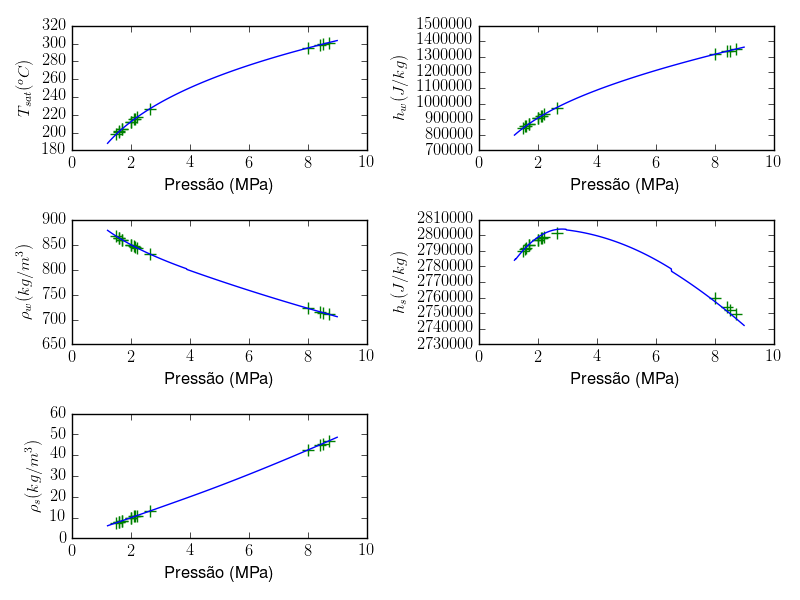
\includegraphics[scale=0.7]{img/steam_table_plots.png}
\end{center}
\legend{As linhas são valores aproximados, enquanto as cruzes
  representam os valores encontrados nas tabelas de vapor saturado}
\end{figure}

O maior erro relativo encontrado foi de cerca de $2,6\%$, mas as
simulações mostraram que esse erro é irrelevante para o comportamento
dinâmico do mesmo.


\subsection{Parâmetros de simulação}

Para a configuração do simulador em relação a uma determinada
caldeira, parâmetros devem ser estimados. Dentre eles, pode-se citar
aspectos geométricos da caldeira e dados da caldeira em seu ponto de
operação ideal. Os tópicos a seguir apresentam uma forma de calcular
tais parâmetros quando em posse de uma caldeira em funcionamento. O
fluxo de cálculo das estimativas foi definido levando em consideração
a dificuldade de se mensurar valores complexos relacionados à
termodinâmica e à geometria da caldeira.

Recomenda-se que os cáculos sejam feitos na ordem em que estão
apresentados, uma vez que as variáveis possuem dependências entre si.

\subsubsection{Gravidade ($g$)}

Esse parâmetro pode ser escolhido arbitrariamente, em torno da
gravidade usual. Os gráficos a seguir mostram as respostas do
simulador a um degrau de $10kg/s$ em $q_s$ para a gravidade entre
$80\%$ e $110\%$ da estimativa original.

\begin{figure}[H]
  \caption{\label{level_resp_g} Respostas do nível a degrau de $10kg/s$
    em $q_s$ para gravidade em variações diferentes}
  \centering
  \subbottom[\label{level_resp_g:80}$80\%$]{
    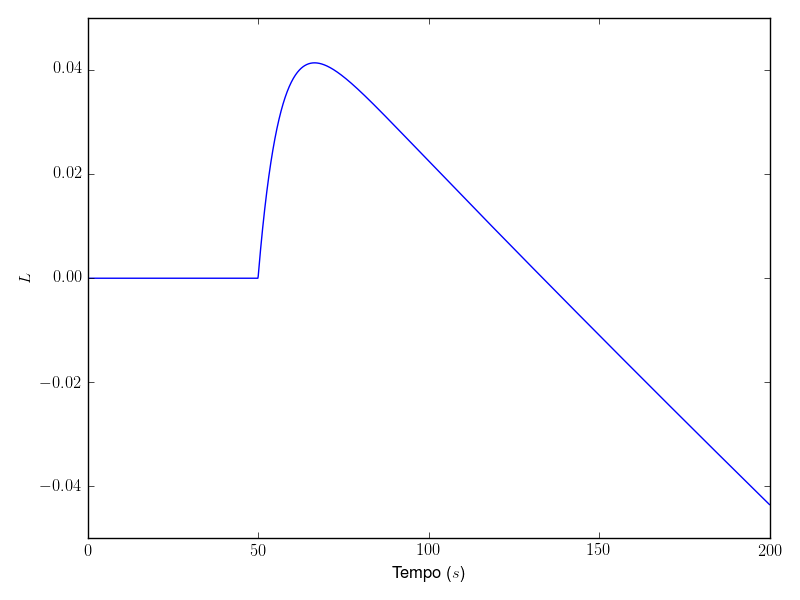
\includegraphics[scale=.25]{img/level_response_test_g_80.png} }
  \subbottom[\label{level_resp_g:90}$90\%$]{
    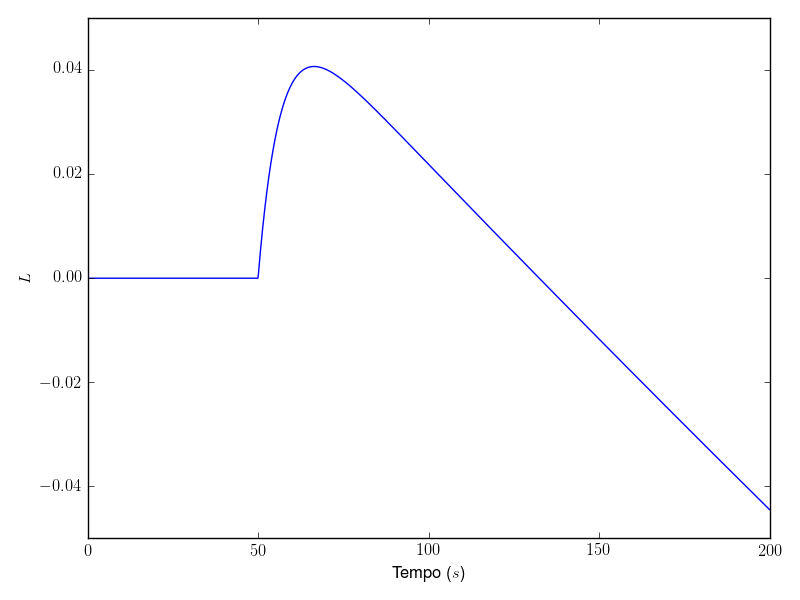
\includegraphics[scale=.25]{img/level_response_test_g_90.png} }
  \subbottom[\label{level_resp_g:110}$110\%$]{
    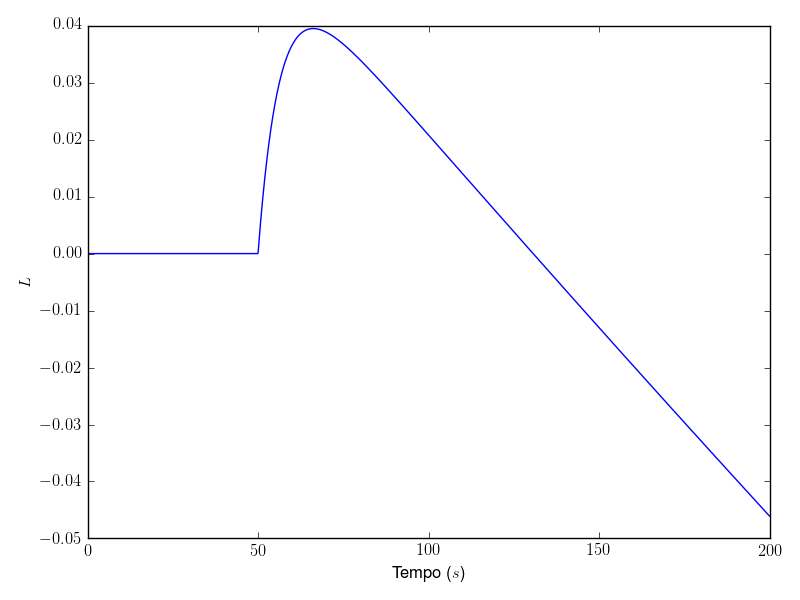
\includegraphics[scale=.25]{img/level_response_test_g_110.png} }
  \subbottom[\label{level_resp_g:120}$120\%$]{
    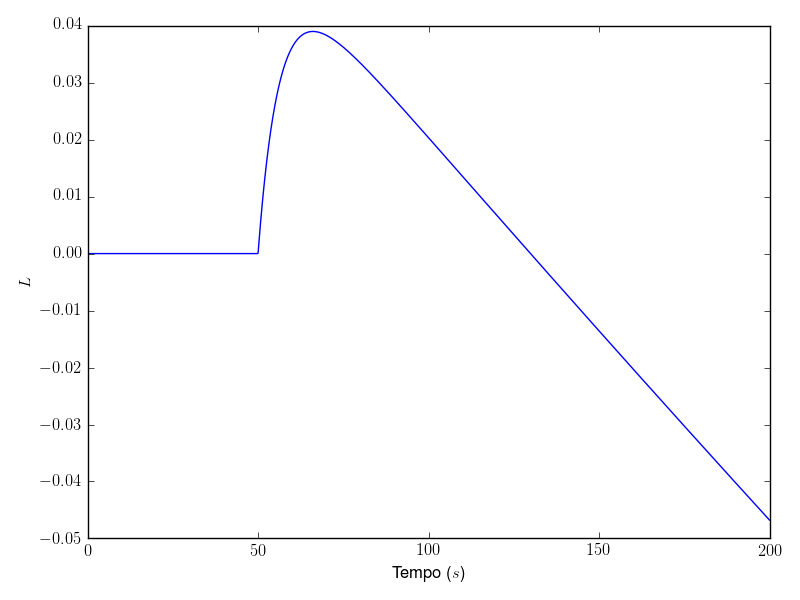
\includegraphics[scale=.25]{img/level_response_test_g_120.png} }
\end{figure}

A seguir, as figuras mostram a resposta de outras variáveis da
caldeira ao mesmo degrau de $10kg/s$ em $q_s$.

\begin{figure}[H]
  \caption{\label{resp_g} Respostas de variáveis de estado a degrau de
    $10kg/s$ em $q_s$ para gravidade em variações diferentes}
  \centering \subbottom[\label{resp_g:80}$80\%$]{
    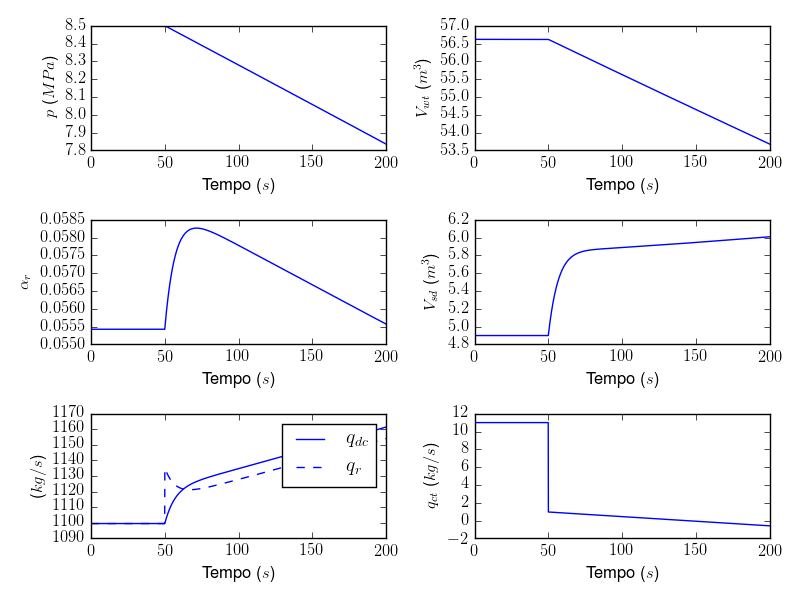
\includegraphics[scale=.25]{img/response_test_g_80.png} }
  \subbottom[\label{resp_g:90}$90\%$]{
    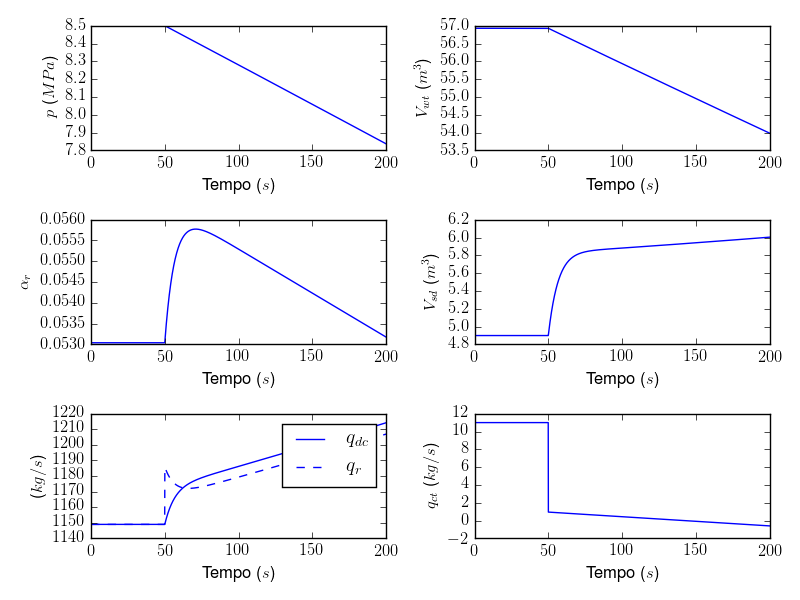
\includegraphics[scale=.25]{img/response_test_g_90.png} }
  \subbottom[\label{resp_g:110}$110\%$]{
    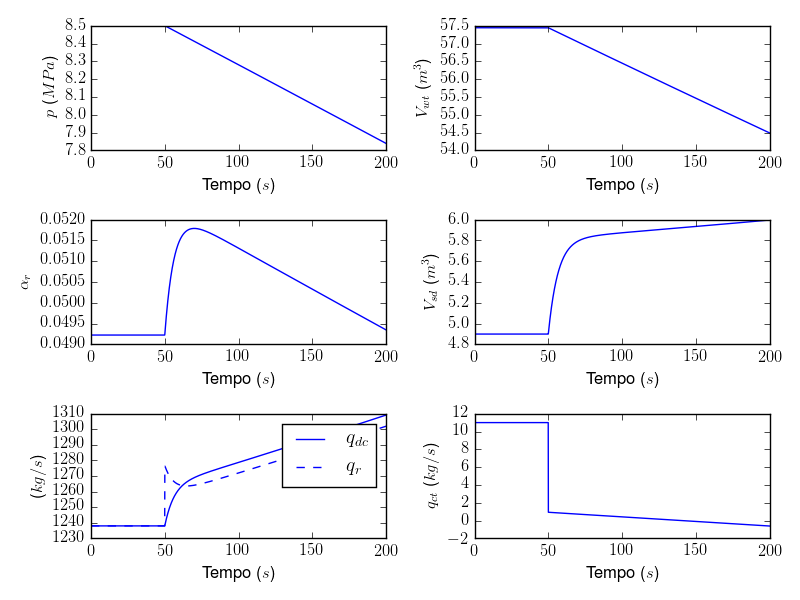
\includegraphics[scale=.25]{img/response_test_g_110.png} }
  \subbottom[\label{resp_g:120}$120\%$]{
    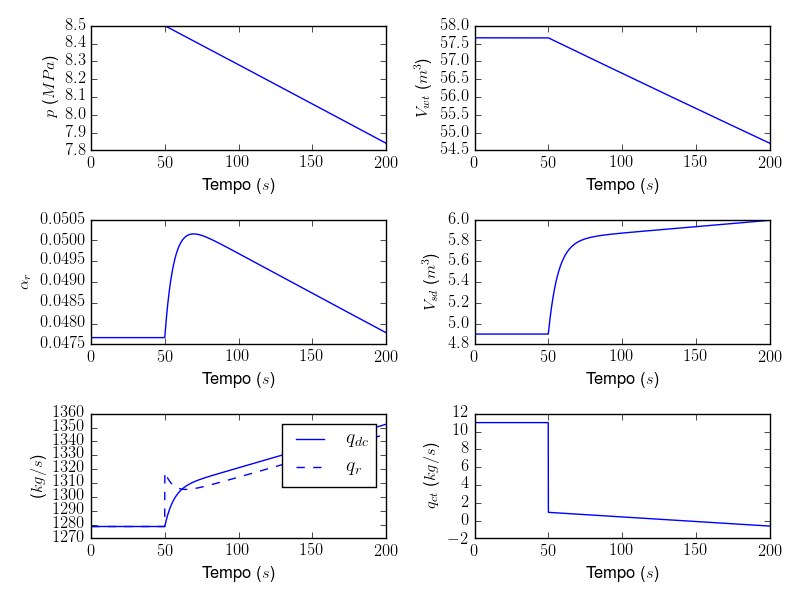
\includegraphics[scale=.25]{img/response_test_g_120.png} }
\end{figure}

Como pode ser visto, a variação do valor da gravidade não afeta em
nada o comportamento dinâmico do sistema. Os valores iniciais são
afetados pois foram estimados inicialmente usando um valor fixo para a
gravidade, porém se os valores iniciais fossem reestimados com a
variação da gravidade, seriam coincidentes com os valores encontrados
em \citeonline{astrom}.

\subsubsection{Entalpia da água de entrada ($h_f$)}

Para baixas temperaturas e altas pressões, as propriedades
termodinâmicas da água são governadas por sua temperatura
\cite{garland2}. No caso das propriedades da água de entrada, pode-se
usar sua temperatura para descobrir a pressão de saturação, através
das aproximações em \citeonline{garland2}. Pode-se então usar essa
pressão de saturação nas aproximações para a água superaquecida,
explicadas em \citeonline{garland}.

\subsubsection{Volume total de água na caldeira ($V_{wt}$)}

Com o valor de $l_o$ obtido da caldeira e o valor inicial de $V_{sd}$
calculado com a equação de $V_{sd}$ no sistema \ref{sistema_geral_rp},
pode-se calcular $V_{wd}$ através da equação \ref{nivel_agua}.

\begin{center}
  $l_o = \dfrac{V_{wd} + V_{sd}}{A_d} \Rightarrow V_{wd} = l_o  A_d -
  V_{sd}$
\end{center}

Com o valor de $V_{wd}$, basta usar a equação \ref{V_wd} para
encontrar $V_{wt}$.



\subsection{Estimativas da caldeira de \citeonline{astrom}}

Além dos parâmetros citados em \citeonline{astrom}, outros são
necessários e foram omitidos em seu trabalho. Tais parâmetros foram
estimados a partir da figura \ref{plots_astrom_step_10kg_qs}.

\begin{figure}[H]
  \caption{\label{plots_astrom_step_10kg_qs} Respostas a incremento de
  $10 kg/s$ na vazão mássica de vapor, a partir de carga média}
  \begin{center}
    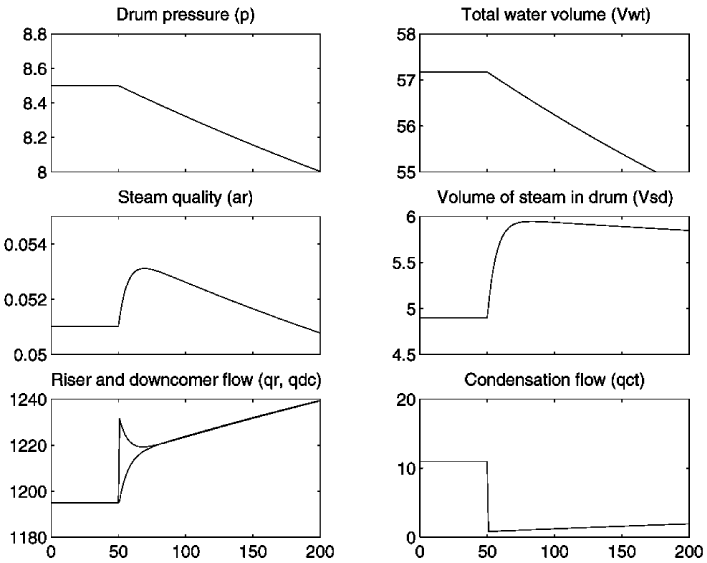
\includegraphics[scale=0.45]{img/plots_astrom_step_q_s_10kg.png}
  \end{center}
  \legend{Fonte: \cite{astrom}. }
\end{figure}

Pode-se retirar da figura os seguintes valores iniciais:
\begin{itemize}
\item $ p = 8,5 MPa $
\item $ V_{wt} = 57,2 m^3 $
\item $ \alpha_r = 0,051 $
\item $ V_{sd} = 4,9 m^3 $
\item $ q_r = q_{dc} = 1190 kg/s $
\item $ q_{ct} = 11 kg/s $
\end{itemize}

Através da pressão inicial e das aproximações das tabelas de vapor
saturado, pode-se calcular o valor das propriedades térmicas da água.

\begin{itemize}
\item $h_s = 2.749.993,696 J/kg$
\item $h_w = 1.340.249,233 J/kg $
\item $h_c = 1.409.744,462 J/kg$
\item $\rho_s = 45,627 kg/m^3$
\item $\rho_w = 713,847 kg/m^3$
\end{itemize}

\subsubsection{Vazão de entrada ($ q_f $)}

Através do sistema de equações \ref{sistema_geral_rp}, pode-se
encontrar o valor de $Q$ inicial, ao utilizar o valor de $h_c$ obtido
das aproximações das tabelas de vapor saturado, juntamente com os
valores de $q_{dc}$ e $\alpha_r$ iniciais observados no gráfico de
\citeonline{astrom}:

$Q = 1195 \times 0,051 \times 1.409.744,4622785489 = 85.916.876,2536
W$

Através do sistema de equações \ref{sistema_geral_rp}, da equação em
regime permanente de $q_{ct}$ e dos valores iniciais obtidos dos
gráficos, pode-se estimar a vazão mássica inicial usada:


\begin{center}
  $Q = q_s h_s - q_f h_f \Rightarrow Q = q_f h_s - q_f h_f$
\end{center}

\begin{equation}  
  q_f h_f = q_f h_s - Q
  \label{qfhf1}
\end{equation}

A partir da equação de $q_{ct}$, tem-se:

\begin{center}
  $q_{ct} = \dfrac{h_w - h_f}{h_c} q_f$

  $q_{ct} h_c = q_f h_w - q_f h_f$
\end{center}

\begin{equation}
  q_f h_f = q_w h_w - q_{ct} h_c
  \label{qfhf2}
\end{equation}

Igualando \ref{qfhf1} e \ref{qfhf2}, obtém-se o valor de $q_f$:

\begin{equation}
  q_f=\dfrac{q_{ct} h_c - Q}{h_w - h_s}
  \label{q_f_init}
\end{equation}

No caso do simulador em questão, esse valor é igual a $q_f = 49,945
kg/s$.

\subsubsection{Entalpia da água de entrada ($h_f$)}

Por não ser mencionada a temperatura da água de entrada em
\citeonline{astrom}, a mesma foi estimada a partir do $Q$ inicial,
substituindo-o na segunda equação do sistema \ref{sistema_geral_rp}.

\begin{center}
  $Q = q_s h_s - q_f h_f \Rightarrow h_f = \dfrac{q_s h_s - Q}{q_f} =
  \dfrac{49.945 \times 2749993,6956 - 85.916.876,2536}{49.945}$
  
  $\therefore h_f = 1.029.763,918 J/kg$
\end{center}

\subsubsection{Área dos tubos descendentes ($A_{dc}$)}

A partir do valor inicial de $\alpha_r$, obtém-se o valor de
$\bar{\alpha}_v$:

\begin{center}
  $\bar{\alpha}_v = 0,2704784 $
\end{center}

Inserindo os valores na equação \ref{Q_lin_sys}, obtém-se o seguinte
valor:

\begin{center}
  $A_{dc} = \dfrac{ k Q^2 }{ 2 \alpha_r^2 h_c^2 \rho_w (\rho_w - \rho_s)
    g \bar{\alpha}_v V_r}  = 0,381657338 m^2$
\end{center}

Os valores iniciais para o restante das variáveis haviam sido
calculados conforme explicado anteriormente, usando as equações de
\ref{sistema_geral_rp} e \ref{Q_lin_sys}.

\subsubsection{Volume de vapor no tubulão para situação hipotética sem
  condensação ($V_{sd}^0)$}

A partir do valor inicial de $V_{sd}$ no gráfico, pode-se estimar o
valor de $V_{sd}^0$ da caldeira ao substituir o valor na equação de
$V_{sd}$ no sistema de equações \ref{sistema_geral_rp}:

\begin{center}
  $V_{sd} = V_{sd}^0 - \dfrac{T_d ( h_w - h_f )} {\rho_s h_c} q_f
  \Rightarrow V_{sd}^0 = V_{sd} + \dfrac{T_d ( h_w - h_f )} {\rho_s
    h_c} q_f$

  $ \therefore V_{sd}^0 = 7,7930138 m^3 $  
\end{center}

\subsubsection{Volume total da caldeira ($V_t$)}

Embora não especificado em \citeonline{astrom}, estima-se que o volume
total da caldeira pode ser representado através dos parâmetros de
entrada do sistema:

\begin{equation}
  V_t = V_d + V_{dc} + V_r = 89 m^3
  \label{V_t_params}
\end{equation}

\subsubsection{Nível da água no ponto de operação ($l_o$)}

Usando o valor inicial de $V_{wt}$, pode-se calcular $V_{wd}$ através
da equação \ref{V_wd}, obtendo um valor de $19,205 m^3$. Sabe-se que,
no ponto de operação, $l=l_w=l_s=0$, então basta usar as equações
\ref{nivel_agua}, \ref{contrib_s_nivel} e \ref{contrib_w_nivel}:

\begin{center}
  $l_{wo} = \dfrac{V_{wd}}{A_d} = 0,9603 m$
  
  $l_{so} = \dfrac{V_{sd}}{A_d} = 0,2450 m$
  
  $l_o = l_{wo} + l_{so} = 1,2053 m$
\end{center}

Para a utilização prática do simulador, esse valor deve ser obtido
através da medição da caldeira original, uma vez que $V_{wd}$ é obtido
através do valor de $l_o$. Esse fluxo de cálculos foi escolhido pois
caldeiras podem ter geometrias complicadas, o que dificulta o cálculo
preciso de volumes \cite{astrom}.

\subsection{Válvula de vazão de água}

Um modelo simples com controle proporcional foi adotado para as
válvulas, eliminando o comportamento instantâneo na mudança de vazão
de vapor e água de alimentação. Também foi adotado um gerador de
distúrbios de acordo com uma distribuição normal. Na figura
\ref{valvulas_step} pode-se ver a resposta do modelo com e sem distúrbio.

\begin{figure}[H]
  \caption{\label{valvulas_step} Resposta do modelo da válvula a um
    degrau de $10kg/s$}
  \centering
  \subbottom[\label{valvulas_step:sem_d} Sem distúrbio]{
    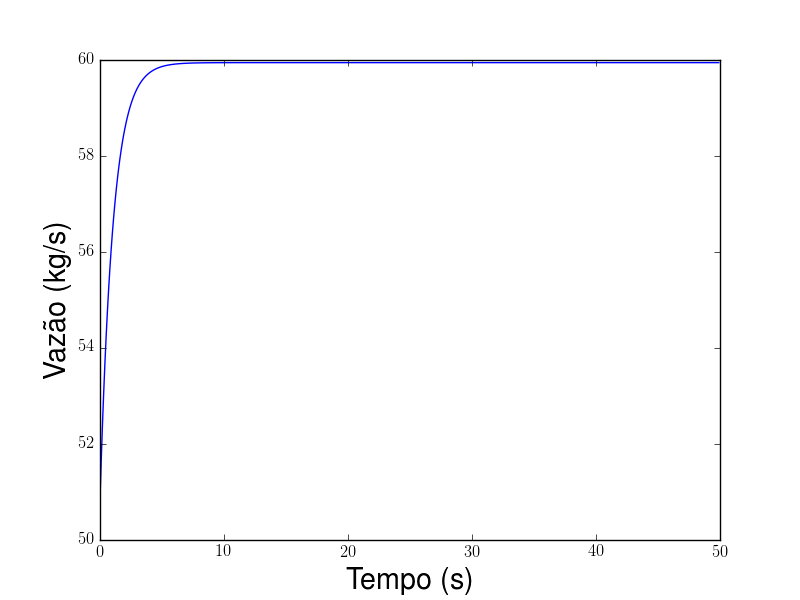
\includegraphics[scale=.25]{img/valve_step_response.png}}
  \subbottom[\label{valvulas_step:com_d} Distúrbio de $\pm 0,3 kg/s$]{
    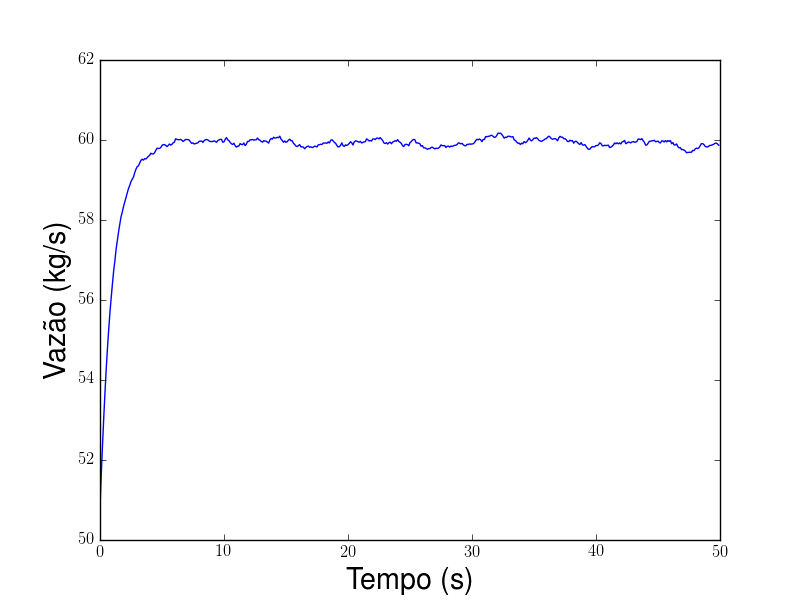
\includegraphics[scale=.25]{img/valve_step_response_biased.png}}
\end{figure}

Claramente uma válvula tem um limite de vazão possível. Para esse
trabalho a vazão máxima escolhida foi de $130,00 kg/s$, levando em
conta os gráficos para a caldeira em operação com carga alta, expostos
em \citeonline{astrom}.

\subsection{Dinâmica da geração de calor}

Para um simulador condizente com a realidade, é necessário simular o
comportamento do sistema para estímulos no fluxo de calor fornecido
para a planta ($Q$). Por se tratar de um comportamento dependente do
modelo dos queimadores da caldeira, o modelo do queimador deve ser
usado, com um sistema de controle próprio. Como a implementação de tal
modelo foge ao escopo do projeto, um simples modelo linear para o
fluxo de calor foi adotado, considerando uma relação linear entre o
fluxo mássico de combustível e o fluxo de calor entregue à caldeira,
apresentado na equação \ref{modelo-calor}. Na fórmula, $k$ foi
escolhido empiricamente, de forma a aproximar-se da constante de tempo
vista nos dados originais obtidos em \citeonline{astrom}. Um valor de
$k = 0,1$ se mostrou satisfatório.

\begin{equation}
  \dot{Q}(t) = Q(t) + k(u - Q(t))
  \label{modelo-calor}
\end{equation}

No caso, $u$ é o ponto de referência para $Q$. Tal modelo causa um
atraso na resposta da $Q$, aproximando-se a modelos de queimadores
reais.

\subsection{Sistemas de controle}

Os dois sistemas de controle principais da caldeira são o controle de
nível e controle de pressão. Como dito em \citeonline{ufrj}, muitas
vezes os dois controles são analisados separadamente, realizando o
ajuste do controle de pressão e depois o ajuste do controle de nível.

\subsubsection{Controle de pressão}

Empiricamente, as seguintes constantes foram adotadas no controlador
PI da pressão:

\begin{equation}
  \begin{cases}
    k_p = 5\times10^6\\
    k_i = 10^7\\
  \end{cases}
  \label{ks_pi_pressao}
\end{equation}

A pressão adotada foi a inicial encontrada nos gráficos em
\citeonline{astrom}, para a caldeira trabalhando com carga média:
$8,5 MPa$.

\subsubsection{Controle de nível}

De acordo com \citeonline{adam1999} e \citeonline{ufrj}, um
controlador PI é suficiente para controlar o nível de água no tubulão,
porém mostra-se complicado o ajuste de tais parâmetros de forma
ótima. Aqui, portanto, usou-se o método prático estabelecido por
\citeonline{ufrj}, que consiste na estimativa empírica dos parâmetros
do controlador após o ajuste do controlador de pressão. Os resultados
do ajuste prático encontram-se a seguir.

\begin{equation}
  \begin{cases}
    k_p=60\\
    k_i=1,2
  \end{cases}
  \label{ks_pid_agua}
\end{equation}

\subsection{Arquitetura de software}

Para se aproximar ao máximo da arquitetura lógica de uma caldeira
real, optou-se por desenvolver um sistema distribuido, em que cada uma
das partes seja facilmente removida. Isso também permite que cada
aplicação seja independente, podendo ser desenvolvida em uma linguagem
diferente da linguagem usada por outras aplicações.

No centro dessa arquitetura, há o simulador do sistema, onde se tem
implementado o modelo da caldeira, assim como os modelos da válvula de
entrada de água e dos queimadores. A implementação desses modelos
podem ser vistos nos anexos \ref{sim_caldeira}, \ref{sim_valvula} e
\ref{sim_queimador}, respectivamente.

O simulador apresenta serviços acessíveis através de sua interface,
onde se pode requisitar os valores de cada variável da caldeira, bem
como alterar valores das mesmas. As variáveis controladas diretamante
através dessa interface são $q_s$, $q_f$ (que na verdade é passada
para o controlador da válvula), e $Q$ (passado para o controlador dos
queimadores), enquanto as variáveis que podem ser lidas são $q_f$,
$q_s$, $Q$, $L$, $P$ e $\alpha_r$. Os anexos \ref{sim_main} e
\ref{sim_thread} mostram o módulo de entrada do simulador e a thread
de controle da simulação.
% TODO: Adicionar apendices

Para fins de testes do simulador, as seguintes aplicações foram
desenvolvidos:
\begin{itemize}
  \item \textbf{Ferramenta de visualização}: Interface gráfica onde
    pode-se ver um gráfico de todas as variáveis disponíveis através
    da interface. A implementação resume-se em um único módulo, que
    pode ser visto no anexo \ref{viewer_main}.
  \item \textbf{Controladores}: Aplicação que implementa os controladores
    de pressão e nível.
\end{itemize}

A aplicação de controladores é constituída do ponto de entrada (módulo
\textit{main}, disponível no anexo \ref{controllers_main}, uma classe
para controle de nível e outra para controle de pressão. Os
controladores usados fazem parte de um módulo de classes de
controladores base, como podem ser vistos em
\ref{controllers_generic}. As classes de controle de nível e controle
de pressão são instanciadas em \textit{main} e realizam o controle
periodicamente, através do método \textit{step}. A implementação de
ambas as classes está disponível nos anexos \ref{controllers_level} e
\ref{controllers_pressure}.


Outro fator de extrema importância em sistemas distribuidos é a
comunicação entre os processos. Para isso, foi usado o
\textit{ZeroMQ}, um MQ que disponibiliza sockets que carregam
mensagens entre processos usando protocolos como TCP/IP, multicast,
entre outros \cite{zmq}. O ZeroMQ possui bibliotecas para várias
linguagens, como C++, Python e Matlab.

Para a aplicação, o protocolo escolhido foi TCP/IP, permitindo a
comunicação entre os módulos do sistema mesmo que não estejam no mesmo
computador. A classe usada para comunicação com o servidor está
disponível no anexo \ref{interface_cliente}, enquanto a classe
de interface usada pelo servidor está disponível no anexo
\ref{interface_servidor}.

A interface do servidor conta com dois canais para troca de mensagens,
um funciona como request-reply e o outro como push-pull.

Através do canal request-reply, clientes solicitam os valores das
variáveis. Uma mensagem de requisição deve conter somente o nome da
variável solicitada.

O canal push-pull recebe comandos de alteração das variáveis, seguindo
o formato ``variável operação valor''. A operação pode ser de adição,
subtração, multiplicação ou divisão, representadas pelos símbolos $+$,
$-$, $*$ e $/$. É importante manter o espaço entre cada parte da
mensagem, ou a mesma é considerada inválida e descartada.

Por precisarem de ferramentas numéricas e de plotagem de gráfico, a
linguagem de programação escolhida foi Python, uma linguagem orientada
a objetos de simples utilização e grande suporte da comunidade. As
ferramentas de plotagem (Matplotlib) e bibliotecas numéricas
(SciPy/NumPy) já são maduras e possuem grande aceitação da comunidade
acadêmica.
